\documentclass[11pt]{article}

\usepackage[a4paper,margin=1in]{geometry}
\usepackage{amsmath,amssymb,amsthm,mathtools}
\usepackage{xcolor}
\usepackage{listings}
\usepackage{hyperref}
\usepackage{enumitem}
\usepackage{mdframed}
\usepackage{booktabs}
\usepackage{tabularx}
\usepackage{titlesec}
\usepackage{parskip}
\usepackage{tikz}
\usetikzlibrary{arrows.meta,positioning,fit,backgrounds,decorations.pathreplacing}

\hypersetup{colorlinks=true, linkcolor=blue!50!black, urlcolor=blue!50!black}

\titlespacing*{\section}{0pt}{16pt}{6pt}
\titlespacing*{\subsection}{0pt}{12pt}{5pt}
\titlespacing*{\subsubsection}{0pt}{9pt}{3pt}
\setlist{nosep, topsep=3pt, itemsep=3pt}
\setlength{\parskip}{6pt}

\definecolor{codebg}{RGB}{243,242,239}
\definecolor{codekeyword}{RGB}{42,120,214}
\definecolor{codecomment}{RGB}{110,110,110}
\lstset{
  basicstyle=\ttfamily\small, backgroundcolor=\color{codebg},
  keywordstyle=\color{codekeyword}\bfseries, commentstyle=\color{codecomment}\itshape,
  frame=single, breaklines=true, showstringspaces=false, tabsize=4,
  columns=flexible, aboveskip=6pt, belowskip=6pt
}

\newmdenv[backgroundcolor=blue!5, linecolor=blue!40!black, linewidth=0.7pt, roundcorner=3pt,
  innermargin=8pt, outermargin=8pt, innertopmargin=6pt, innerbottommargin=6pt, skipabove=8pt, skipbelow=8pt]{cbox}
\newmdenv[backgroundcolor=green!6, linecolor=green!35!black, linewidth=0.7pt, roundcorner=3pt,
  innermargin=8pt, outermargin=8pt, innertopmargin=6pt, innerbottommargin=6pt, skipabove=8pt, skipbelow=8pt]{keyidea}
\newmdenv[backgroundcolor=gray!7, linecolor=gray!50!black, linewidth=0.6pt, roundcorner=2pt,
  innermargin=8pt, outermargin=8pt, innertopmargin=6pt, innerbottommargin=6pt, skipabove=8pt, skipbelow=8pt]{recap}
\newmdenv[backgroundcolor=orange!8, linecolor=orange!50!black, linewidth=0.6pt, roundcorner=2pt,
  innermargin=8pt, outermargin=8pt, innertopmargin=6pt, innerbottommargin=6pt, skipabove=8pt, skipbelow=8pt]{stepbox}

\title{\textbf{fracmem} --- Full Architecture, Explained From Zero\\[0.4em]
\large How a Fractional-Order Derivative Becomes a Fixed-Cost, Fixed-Memory Recursive Filter}
\author{}
\date{\today}

\begin{document}
\maketitle

\begin{cbox}
\textbf{What this document is.} A complete, from-scratch walkthrough of the \texttt{fracmem} library exactly as it exists in this repository (\texttt{fracmem\_pypi/src/fracmem}, version 0.2.0) --- what problem it solves, the mathematics behind the solution, how that mathematics maps line-by-line onto the four source files, a small worked numerical example you can trace by hand, and real measured results from actually running the code. No prior knowledge of fractional calculus is assumed.
\end{cbox}

\tableofcontents

%=================================================================
\section{Notation --- every symbol used in this document, defined once}

Before any mathematics, here is what every letter means in plain English. Keep this page open; every later section reuses exactly these symbols with exactly these meanings.

\begin{center}
\small
\begin{tabularx}{\textwidth}{lX}
\toprule
Symbol & Meaning \\
\midrule
\textbf{signal} & The stream of numbers you are measuring over time --- e.g.\ a sensor reading taken over and over. In code this is just an array/list of numbers. \\
$x$ & The signal itself, written as a sequence of samples $x_0, x_1, x_2, \dots$ \\
$k$ & The \textbf{sample index} --- which measurement you're on. $k=0$ is the very first sample ever taken, $k=1$ is the second, and so on. $k$ is just a counter; it is \emph{not} a physical time in seconds by itself. \\
$x_k$ (also written $x(t_k)$) & The value of the signal at sample number $k$ --- ``the $k$-th measurement.'' \\
$h$ & The \textbf{sample time}: how many seconds (or whatever your time unit is) pass between one sample and the next. If your sensor reports 100 times per second, $h=0.01$ seconds. $h$ converts ``sample counts'' into real time: the actual time of sample $k$ is $t_k = k\cdot h$. \\
$D^\alpha x(t_k)$ & ``The fractional derivative of $x$, of order $\alpha$, evaluated at sample $k$'' --- the single number this whole library exists to compute cheaply. For $\alpha=1$ this is just the ordinary derivative (rate of change); for other $\alpha$ (e.g.\ $0.5$) it is the fractional generalization defined in the next section. \\
$\alpha$ & The \textbf{fractional order} itself --- a number you choose (e.g.\ $0.5$) that says which fractional derivative you want. It is a fixed setting, not something computed from the data. \\
$j$ & A second counter, used only for ``how many samples back am I looking'': $j=0$ means the current sample, $j=1$ means one sample ago, $j=2$ means two samples ago, etc. So the term $w_j\,x_{k-j}$ means ``the weight for looking $j$ samples back, times the value that was seen $j$ samples back from the current sample $k$.'' \\
$w_j$ & The \textbf{GL weight} for looking $j$ samples into the past --- a fixed number (depends only on $\alpha$ and $j$, never on the signal) that says how much sample $x_{k-j}$ contributes to today's derivative estimate. \\
$L$ & The \textbf{local window length} --- how many of the most recent samples ($j=0,\dots,L-1$) get treated \emph{exactly}, with no approximation at all. A setting you choose, e.g.\ $L=32$. \\
$p$ & The \textbf{number of ``leaky buckets''} (exponential modes) used to approximate everything older than $L$ samples. A setting you choose, e.g.\ $p=16$. \\
$i$ & An index over the buckets: $i=1,\dots,p$ (or $0,\dots,p-1$ in code) --- ``which bucket am I talking about.'' \\
$\lambda_i$ & The \textbf{decay (leak) rate} of bucket $i$ --- a number between 0 and 1. Every sample, bucket $i$'s stored value is multiplied by $\lambda_i$ (so a fraction $1-\lambda_i$ ``leaks away'') before the new sample is added in. Computed once from pure math (Section~3); never touched by data afterward. \\
$c_i$ & The \textbf{combination weight} of bucket $i$ --- how much bucket $i$'s current reading counts toward the final tail estimate. This is the \emph{only} quantity in the whole method that gets adjusted using real training data. \\
$m_i[k]$ & The current \textbf{state (stored value)} of bucket $i$ after sample $k$ has been processed --- a single running number, updated every sample, never an array. \\
$x_{\text{delayed}}[k]$ & The signal shifted right by $L$ samples (and zero for the first $L$ samples) --- this is what actually gets fed into the buckets, since the buckets are only responsible for everything \emph{older} than the $L$-sample local window. \\
$\text{local}[k]$ & The exact contribution of the most recent $L$ samples to the derivative at sample $k$ (Step~3 below). \\
$\text{tail}[k]$ & The buckets' combined estimate of the contribution from everything \emph{older} than $L$ samples (Step~7 below). \\
$\text{gold}[k]$ & The \emph{exact}, textbook fractional derivative at sample $k$, computed the slow, unbounded-memory way --- the ``ground truth'' every approximation in this document is checked against. \\
$\text{approx}[k]$ & What the compressed filter actually outputs: $\text{approx}[k] = \text{local}[k] + \text{tail}[k]$. \\
\bottomrule
\end{tabularx}
\end{center}

\begin{cbox}
\textbf{A concrete example of $k$, $j$, and $w_j x_{k-j}$, before anything else.} Suppose your signal is just six numbers, indexed $k=0,1,2,3,4,5$:
\[
x = [\,x_0,x_1,x_2,x_3,x_4,x_5\,] = [\,5,\ 3,\ 8,\ 1,\ 9,\ 2\,].
\]
Say you want the derivative estimate \emph{at sample $k=3$} (the sample whose value is $x_3=1$). The formula $\sum_j w_j x_{k-j}$ means: look backward from sample $3$, one step of $j$ at a time, multiply each sample you land on by its weight $w_j$, and add them all up.

\begin{center}
\small
\begin{tabular}{c c c c c}
\toprule
$j$ (samples back) & index landed on $=k-j=3-j$ & value $x_{k-j}$ & weight $w_j$ & product $w_j x_{k-j}$ \\
\midrule
$j=0$ (current sample itself) & $3-0=3$ & $x_3=1$ & $w_0=1.000000$ & $1.000000\times1=1.000000$ \\
$j=1$ (one sample ago) & $3-1=2$ & $x_2=8$ & $w_1=-0.500000$ & $-0.500000\times8=-4.000000$ \\
$j=2$ (two samples ago) & $3-2=1$ & $x_1=3$ & $w_2=-0.125000$ & $-0.125000\times3=-0.375000$ \\
$j=3$ (three samples ago) & $3-3=0$ & $x_0=5$ & $w_3=-0.062500$ & $-0.062500\times5=-0.312500$ \\
\bottomrule
\end{tabular}
\end{center}

The sum can't go back any further than $j=3$ here, simply because sample $k=3$ only \emph{has} 4 samples behind it (indices $0,1,2,3$) --- there is no $x_{-1}$. Adding the product column: $1.000000-4.000000-0.375000-0.312500=-3.687500$. With $h=1$ (so $h^{-\alpha}=1$, see Section~2), that product sum \emph{is} the answer:
\[
D^{0.5}x(t_3) \approx -3.687500.
\]
That's the entire formula from Section~2 --- $j$ is nothing more than ``how many steps backward am I looking right now,'' and $w_j\,x_{k-j}$ is ``grab the sample $j$ steps back, scale it by that step's fixed weight.'' Every occurrence of $j$, $w_j$, and $x_{k-j}$ anywhere later in this document means exactly this, just with $\alpha=0.5$'s specific weights and a longer signal.
\end{cbox}

\section{The problem, from zero}

\subsection{An ordinary derivative}
An ordinary derivative of a signal $x(t)$ tells you how fast $x$ is changing \emph{right now}. To compute it you only ever need the current value and the value just before it: $\dot x(t_k) \approx \frac{x(t_k)-x(t_{k-1})}{h}$ (recall: $t_k=k\cdot h$ is the actual time of sample $k$, and $h$ is the fixed time gap between samples). One subtraction, one division. The past beyond one step back is irrelevant.

\subsection{A fractional derivative}
A \textbf{fractional-order derivative} $D^\alpha x$, for a non-integer order like $\alpha=0.5$ (a ``half derivative''), is a generalization that shows up naturally in fractional-order PID control, viscoelastic material models, and battery impedance models. The standard (Gr\"unwald--Letnikov, ``GL'') definition is:
\[
D^\alpha x(t_k) \;\approx\; h^{-\alpha} \sum_{j=0}^{k} w_j\, x_{k-j},
\qquad w_0 = 1,\quad w_j = w_{j-1}\!\left(1 - \frac{1+\alpha}{j}\right).
\]
Unlike the ordinary derivative, \textbf{every single past sample $x_{k-j}$ contributes}, weighted by $w_j$. The weights decay, but only as a power law, $w_j \sim j^{-\alpha-1}$ --- much slower than the geometric decay you get from an ordinary filter. You cannot just chop the sum off after a few terms without throwing away real accuracy.

\subsection{Why that is a practical dealbreaker}
Two consequences of ``every past sample matters, forever'':
\begin{itemize}
\item \textbf{Memory} needed to compute $D^\alpha x(t_k)$ exactly grows with $k$ --- you must keep the whole history.
\item \textbf{Compute} per new sample also grows with $k$ --- the sum has $k{+}1$ terms.
\end{itemize}
On a laptop analysing a finite recording, that is merely slow. On an embedded controller, a drone, or any real-time loop that runs indefinitely, it is not implementable: memory and CPU budgets are fixed, but the exact computation's cost is not.

\begin{recap}
\textbf{In short:} fractional derivatives are useful, but computing them exactly needs unbounded memory and unbounded work per sample as the signal runs longer. \texttt{fracmem} exists to remove exactly that restriction, while telling you in advance how much accuracy you gave up.
\end{recap}

%=================================================================
\section{The core idea}

\subsection{Split the sum in two}
Pick a window length $L$ (e.g.\ 32). Split the infinite sum at $j=L$:
\[
D^\alpha x(t_k) \;=\; \underbrace{h^{-\alpha}\!\!\sum_{j=0}^{L-1} w_j x_{k-j}}_{\text{local: exact, no approximation}} \;+\; \underbrace{h^{-\alpha}\!\!\sum_{j=L}^{k} w_j x_{k-j}}_{\text{tail: this is what gets compressed}}.
\]
The \textbf{local} part is an ordinary length-$L$ FIR filter on the $L$ most recent samples. It is never approximated by anything in this library --- it is computed exactly, every time.

\subsection{Replace the tail with a handful of leaky buckets}
The tail still nominally needs every sample back to $j=k$. Here is the trick: instead of a power-law decay ($w_j \sim j^{-\alpha-1}$, which needs to be tracked exactly to stay accurate over a long range), approximate the tail kernel by a short \textbf{sum of $p$ exponentials}:
\[
w_j \;\approx\; \sum_{i=1}^{p} c_i\, \lambda_i^{\,j-L}, \qquad j \ge L .
\]
Each exponential term $\lambda_i^{\,j-L}$ can be tracked with a single running number $m_i$, updated by \emph{one multiply and one add per new sample}:
\[
m_i[k] = \lambda_i\, m_i[k-1] + x_{k-L}, \qquad \text{tail}[k] = \sum_{i=1}^p c_i\, m_i[k].
\]
This is the classical \textbf{Sum-of-Exponentials (SOE)} technique. Think of each $m_i$ as a leaky bucket: every new (delayed) sample is poured in, and a fixed fraction $\lambda_i$ of whatever is already in the bucket survives to the next step. A handful of buckets with different leak rates, added together with the right weights $c_i$, closely mimics the slow long-range decay of the exact tail --- without ever storing an individual old sample.

\begin{center}
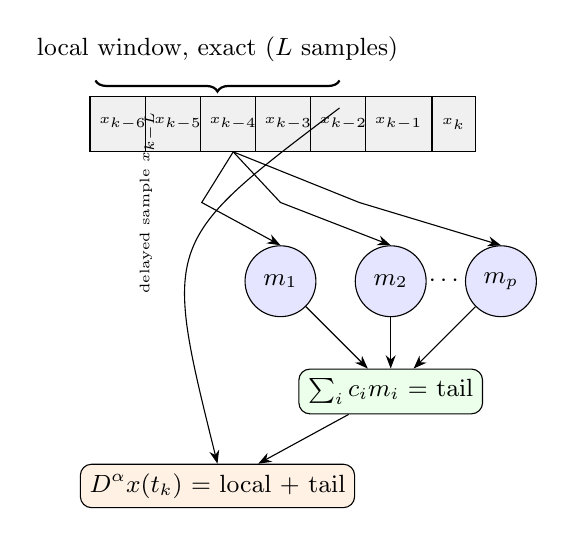
\begin{tikzpicture}[
  every node/.style={font=\small},
  sig/.style={draw, minimum height=0.7cm, minimum width=0.55cm, fill=gray!12},
  bucket/.style={draw, circle, minimum size=0.9cm, fill=blue!10},
  >=Stealth
]
  \foreach \i/\lab in {0/x_{k-6},1/x_{k-5},2/x_{k-4},3/x_{k-3},4/x_{k-2},5/x_{k-1},6/x_{k}}
    \node[sig] (s\i) at (\i*0.7,0) {\tiny $\lab$};
  \draw[decorate,decoration={brace,amplitude=4pt},thick] (2.75,0.55) -- (-0.35,0.55)
    node[midway,above=3pt]{local window, exact ($L$ samples)};

  \node[bucket] (b1) at (2.0,-2.0) {$m_1$};
  \node[bucket] (b2) at (3.4,-2.0) {$m_2$};
  \node[bucket] (b3) at (4.8,-2.0) {$m_p$};
  \node at (4.1,-2.0) {$\cdots$};

  \draw[->] (s2.south) -- (1.0,-1.0) -- (b1.north);
  \draw[->] (s2.south) -- (2.0,-1.0) -- (b2.north);
  \draw[->] (s2.south) -- (3.0,-1.0) -- (b3.north);
  \node[above,rotate=90,font=\tiny] at (0.55,-1.0) {delayed sample $x_{k-L}$};

  \node[draw,rounded corners,fill=green!8,minimum width=2.3cm] (sum) at (3.4,-3.4) {$\sum_i c_i m_i$ = tail};
  \draw[->] (b1) -- (sum);
  \draw[->] (b2) -- (sum);
  \draw[->] (b3) -- (sum);

  \node[draw,rounded corners,fill=orange!10] (out) at (1.2,-4.6) {$D^\alpha x(t_k)$ = local + tail};
  \draw[->] (2.75,0.2) .. controls (0.5,-1.5) .. (out.north);
  \draw[->] (sum) -- (out);
\end{tikzpicture}
\end{center}

\begin{keyidea}
\textbf{Why this matters:} once fitted, the entire ``distant past'' is compressed to $p$ numbers ($m_1,\dots,m_p$), each updated with one multiply-add per new sample. Total deployed cost is $O(L+p)$ compute and $O(p)$ persistent memory, per sample, \emph{forever} --- independent of how long the signal has been running.
\end{keyidea}

\subsection{Where $\lambda_i$ (the leak rates) come from --- pure math, no data}
The decay rates $\lambda_i$ are not guessed and not fit to any signal. They come from an exact Gamma-function integral identity for the power-law kernel (proved in the accompanying theory document):
\[
j^{-\beta} = \frac{1}{\Gamma(\beta)} \int_0^\infty s^{\beta-1} e^{-sj}\, ds, \qquad \beta = \alpha + 1,
\]
discretized by log-spaced quadrature into $p$ nodes $s_i$, giving $\lambda_i = e^{-s_i}$. This step uses \textbf{zero signal data} --- it is computed once, offline, directly from $\alpha$ and $L$.

\subsection{Where data comes in --- only the final weights}
After $\lambda_i$ is fixed, one knob remains: how much weight $c_i$ to give each bucket when summing them. \texttt{fracmem} tunes \emph{only} this small set of weights using a handful of representative training signals, via cross-validated ridge regression --- a small, convex, numerically well-posed least-squares problem. Because $\lambda_i$ is never re-fit, the fitting problem stays easy and stable; refitting the decay rates themselves from data would instead be an ill-posed, non-convex problem.

\begin{recap}
\textbf{In short:} exact math (a Gamma-function identity) fixes \emph{how fast} each bucket leaks; a small amount of data only tunes \emph{how much weight} each bucket gets in the final sum. That separation is what lets the library certify a worst-case error bound before ever seeing real data.
\end{recap}

%=================================================================
\section{Step by step: the math as it is actually implemented}

Each step below corresponds to one function in the source tree \texttt{fracmem\_pypi/src/fracmem/}.

\begin{stepbox}
\textbf{Step 1 --- Exact GL weights.} \texttt{kernel.gl\_weights(alpha, n)} computes $w_0,\dots,w_{n-1}$ via the stable recursion $w_j = w_{j-1}(1-\tfrac{1+\alpha}{j})$ (never evaluating the Gamma function directly, which would suffer large cancellation errors for many $j$).
\end{stepbox}

\begin{stepbox}
\textbf{Step 2 --- The exact reference.} \texttt{kernel.full\_gl\_derivative} convolves the signal against the \emph{full} weight sequence. This is the ``gold standard'' target the whole library exists to approximate cheaply --- $O(n)$ cost per new sample, used only for validation, never deployed.
\end{stepbox}

\begin{stepbox}
\textbf{Step 3 --- The local exact window.} \texttt{kernel.local\_exact\_term(x, alpha, h, L, w)} convolves against only the first $L$ weights: an ordinary length-$L$ FIR filter, exact, no approximation.
\end{stepbox}

\begin{stepbox}
\textbf{Step 4 --- Quadrature nodes.} \texttt{soe.soe\_nodes\_and\_weights(alpha, L, m\_max, p)} discretizes the Gamma-integral identity on a log-spaced grid from $s_{\min}=1/m_{\max}$ to $s_{\max}=8$ (past $e^{-8}$ per sample the contribution is already below any meaningful noise floor), returning $p$ pairs $(\lambda_i, c_i^{(0)})$. Pure math, no data.
\end{stepbox}

\begin{stepbox}
\textbf{Step 5 --- Refit weights to the exact kernel.} \texttt{soe.soe\_refit\_weights} solves a small least-squares problem so the sum of exponentials matches the \emph{exact GL tail weights themselves} (not any signal) as closely as possible near $j=L$, correcting the small mismatch between the asymptotic power law and the true kernel. Still zero signal data.
\end{stepbox}

\begin{stepbox}
\textbf{Step 6 --- Certified error bound.} \texttt{soe.soe\_tail\_error} evaluates the worst-case relative error of the $(\lambda,c)$ reconstruction against the exact tail weights, at log-spaced probe points. Because this only compares math to math, it can be computed \emph{before} the filter ever sees a real signal. \texttt{soe.adaptive\_soe\_tail\_kernel} uses this to auto-grow $p$ until a target tolerance is met.
\end{stepbox}

\begin{stepbox}
\textbf{Step 7 --- The deployed recursion.} \texttt{filter.diagonal\_recurrence} implements $m_i[k]=\lambda_i m_i[k-1]+x_{k-L}$, $\text{out}[k]=\sum_i c_i m_i[k]$ --- $p$ independent one-line recursions. This exact recursion is what \texttt{.step()}, \texttt{.predict()}, and the MicroPython export all ultimately run.
\end{stepbox}

\begin{stepbox}
\textbf{Step 8 --- Data enters here, and only here.} \texttt{filter.mode\_features} computes every bucket's trajectory on the training signals; \texttt{filter.ridge\_solve\_c} solves $c^\star=(FF^\top+\text{reg}\cdot\text{diag})^{-1}Ft$ (energy-scaled ridge regression); \texttt{filter.cv\_select\_reg} picks the regularization strength by honest $k$-fold cross-validation restricted to the training signals. The output replaces the analytical $c$ from Step 5 with a data-refined $c$ --- $\lambda_i$ itself is never touched again.
\end{stepbox}

\begin{stepbox}
\textbf{Step 9 --- Assemble.} \texttt{filter.CompressedFractionalFilter.fit(...)} runs Steps 4--8 once, offline. \texttt{.predict(...)} and \texttt{.step(...)} run Steps 3+7 (local + tail) forever after, at fixed $O(L+p)$ cost.
\end{stepbox}

\subsection{One more subtlety: three derivative ``definitions''}
The GL discretization above, applied directly to a causal signal ($x(t){=}0$ for $t{<}0$), is numerically identical to the \textbf{Riemann--Liouville (RL)} derivative --- \texttt{kernel.rl\_derivative} is literally an alias for \texttt{full\_gl\_derivative}. The \textbf{Caputo} derivative instead removes the singularity a nonzero initial value would introduce, by applying the same machinery to $x(t)-x(0)$: \texttt{kernel.caputo\_derivative} and \texttt{filter.\_apply\_definition} implement exactly that one subtraction, then defer to the ordinary GL/RL path.

%=================================================================
\section{A worked example you can trace by hand}

To make every number concrete, here is a tiny, deliberately small configuration: $\alpha=0.5$, $h=1$, local window $L=4$, $p=4$ buckets, run on a 24-sample unit-step signal ($x_k=1$ for all $k$). This is small enough to print every intermediate quantity in full; Section~5 then shows results at the library's normal, realistic scale.

\subsection{The exact GL weights}
Using the recursion from Step 1 (only the first 10 of 24 shown):
\[
w = [\,1,\ -0.5,\ -0.125,\ -0.0625,\ -0.03906,\ -0.02734,\ -0.02051,\ -0.01611,\ -0.01309,\ -0.01091,\ \dots\,]
\]

\subsection{Design the tail (pure math, before any data)}
With $L=4$ and $p=4$, Steps 4--5 give:
\[
\lambda = [\,0.9100,\ 0.7151,\ 0.3034,\ 0.0144\,], \qquad
c = [\,-0.0141,\ -0.0103,\ -0.0314,\ 0.1208\,].
\]
Notice the spread: $\lambda_1{=}0.91$ decays slowly (a ``long-memory'' bucket), $\lambda_4{=}0.014$ decays almost immediately (a ``short-memory'' bucket) --- together they span the range of decay speeds needed to mimic the power-law tail.

\subsection{Run the filter, sample by sample}
The delayed input $x_{k-L}$ is zero for $k<L$ (the tail has nothing to contribute until the local window has consumed its first $L$ samples), then becomes $1$ from $k=L$ onward. Table~\ref{tab:trace} shows the full trace.

\begin{table}[h]
\centering
\caption{Full worked trace: exact reference (\texttt{gold}) vs.\ the compressed filter (\texttt{local + tail}).}
\label{tab:trace}
\small
\begin{tabular}{rrrrrr}
\toprule
$k$ & gold (exact) & local & tail & approx & abs.\ error \\
\midrule
0  & 1.00000 & 1.00000 & 0.00000 & 1.00000 & 0.0e+00 \\
1  & 0.50000 & 0.50000 & 0.00000 & 0.50000 & 0.0e+00 \\
2  & 0.37500 & 0.37500 & 0.00000 & 0.37500 & 0.0e+00 \\
3  & 0.31250 & 0.31250 & 0.00000 & 0.31250 & 0.0e+00 \\
4  & 0.27344 & 0.31250 & 0.06497 & 0.37747 & 1.04e-01 \\
5  & 0.24609 & 0.31250 & 0.03698 & 0.34948 & 1.03e-01 \\
6  & 0.22559 & 0.31250 & 0.01717 & 0.32967 & 1.04e-01 \\
8  & 0.19638 & 0.31250 & -0.01073 & 0.30177 & 1.05e-01 \\
12 & 0.16118 & 0.31250 & -0.04656 & 0.26594 & 1.05e-01 \\
16 & 0.13995 & 0.31250 & -0.06894 & 0.24356 & 1.04e-01 \\
20 & 0.12537 & 0.31250 & -0.08373 & 0.22877 & 1.03e-01 \\
23 & 0.11700 & 0.31250 & -0.09158 & 0.22092 & 1.04e-01 \\
\bottomrule
\end{tabular}
\end{table}

Two things to notice, exactly as the design predicts:
\begin{itemize}
\item For $k<L$, \texttt{local} alone equals \texttt{gold} exactly (the tail has not switched on yet) and \texttt{tail}$=0$.
\item From $k=L$ onward, \texttt{local} freezes at its $k{=}L{-}1$ value (it only ever sees the same most-recent $L$ constant samples), and \texttt{tail} takes over tracking the slow decay of the rest of the sum.
\end{itemize}

\subsection{The bucket state trace}
Underneath \texttt{tail}, here is exactly what the $p{=}4$ leaky buckets are doing, sample by sample, once the delayed input switches on at $k=4$:
\begin{center}
\small
\begin{tabular}{rrl}
\toprule
$k$ & $x_{k-L}$ & bucket state $m=[m_1,m_2,m_3,m_4]$ \\
\midrule
4 & 1 & $[1.000,\ 1.000,\ 1.000,\ 1.000]$ \\
5 & 1 & $[1.910,\ 1.715,\ 1.303,\ 1.014]$ \\
6 & 1 & $[2.738,\ 2.227,\ 1.396,\ 1.015]$ \\
7 & 1 & $[3.492,\ 2.592,\ 1.423,\ 1.015]$ \\
\bottomrule
\end{tabular}
\end{center}
Each new column is $m_i[k]=\lambda_i m_i[k-1]+x_{k-L}$ (Step 7) --- exactly one multiply and one add per bucket, no history array involved.

\subsection{The certified bound, checked against reality}
Step 6's offline bound (computed purely from $\alpha$, $L$, $\lambda$, $c$ --- never touching this specific signal) reports a worst-case relative tail error of \textbf{11.7\%} for this tiny $(L{=}4,p{=}4)$ configuration. The error actually observed on this demo signal is \textbf{10.3--10.5\%} at every point past $k=L$. The bound is not just close, it is doing exactly its job: predicting, in advance, the right order of magnitude of error this filter will have on a signal it has never seen. This is only a 4-bucket, tiny-budget demo, deliberately chosen to be small enough to print by hand; Section~5 shows what happens once $L$ and $p$ are set to the library's normal working sizes.

%=================================================================
\section{Results at realistic scale}

The numbers above use a deliberately tiny budget so every value could be printed. Run at the sizes the library is actually meant for ($\alpha=0.5$, $L=32$, $p=16$, fit on 8 training signals of 3000 samples each) and measured directly from \texttt{examples/basic-usage.py} in this repository:

\begin{table}[h]
\centering
\caption{Measured on this repository's environment: compressed filter vs.\ exact reference.}
\begin{tabular}{lrr}
\toprule
Signal length & fracmem \texttt{.predict()} & exact reference (unbounded memory) \\
\midrule
50,000 samples & 100.4 ms & 1998.0 ms \\
\bottomrule
\end{tabular}
\end{table}

On this 50,000-sample test signal (well beyond the 3,000-sample training signals), \textbf{fracmem tracks the exact reference to 1.15\% relative RMSE}, roughly \emph{ten times} more accurate than the tiny hand-worked example above, simply because $L{=}32,p{=}16$ gives the tail far more room to represent the true kernel than $L{=}4,p{=}4$ did.

\subsection{Accuracy is a direct, controllable trade against deployed cost}
\texttt{CompressedFractionalFilter.auto(alpha, h, tol=\dots)} grid-searches $(L,p)$ cheapest-first and returns the smallest filter meeting a target accuracy. Measured directly from \texttt{examples/auto-params.py} in this repository:

\begin{table}[h]
\centering
\caption{Measured: target accuracy vs.\ the cheapest filter that achieves it.}
\begin{tabular}{rrrrr}
\toprule
target RMSE & $L$ & $p$ & mult-adds / sample & achieved RMSE \\
\midrule
$10^{-2}$ & 8 & 4  & 12 & $5.65\times10^{-3}$ \\
$10^{-3}$ & 8 & 8  & 16 & $2.27\times10^{-4}$ \\
$10^{-4}$ & 8 & 16 & 24 & $8.65\times10^{-7}$ \\
\bottomrule
\end{tabular}
\end{table}

\subsection{Why the exact reference eventually always loses}
fracmem's per-sample cost is fixed ($L{+}p$ multiply-adds), so total time grows \emph{linearly} with signal length. The exact reference recomputes a longer convolution sum on every new sample, so its cost grows \emph{quadratically}. The crossover --- the point past which fracmem is the faster option --- happens well before 20,000 samples in this repository's measurements, and the gap widens without bound as the signal gets longer. This is the entire point of the library: the trade only gets more favorable the longer the deployment runs.

\subsection{Test suite}
Every mechanism described in this document has a dedicated automated test. Running the full suite in this repository:
\begin{lstlisting}[language=bash]
$ pytest tests/ -q
................................                               [100%]
32 passed in 1.54s
\end{lstlisting}
covering: the core filter and both weight-fit paths, streaming-vs-batch numerical equivalence, adaptive tail construction, automatic $(L,p)$ search, save/load round-tripping, all three derivative definitions, the no-training-data construction from Section~\ref{sec:no-training-data} (including that \texttt{tail\_fit\_points} actually changes the result), the exported MicroPython runtime checked against the desktop implementation, and the plain-C runtime (Section~\ref{sec:c-runtime}) compiled with \texttt{gcc} and checked against the same desktop implementation.

%=================================================================
\section{The four source files, and what each one owns}

\begin{center}
\small
\begin{tabularx}{\textwidth}{lX}
\toprule
File & Responsibility \\
\midrule
\texttt{kernel.py} & The exact GL/RL/Caputo target (Steps 1--3). What the library approximates, and the reference it is validated against. Zero approximation lives here. \\
\texttt{soe.py} & The Sum-of-Exponentials tail construction (Steps 4--6): decay rates from the Gamma-integral identity, weight refit against the exact kernel, and the certified offline error bound. Zero signal data ever enters this file. \\
\texttt{filter.py} & The deployed recursion (Step 7), the data-driven weight fit (Step 8), and the \texttt{CompressedFractionalFilter} class tying it all together: \texttt{.fit()}, \texttt{.predict()}, \texttt{.step()}/\texttt{.reset\_stream()}, \texttt{.save()}/\texttt{.load()}, \texttt{.auto()}, and \texttt{.from\_analytic()} (Section~\ref{sec:no-training-data}). \\
\texttt{embedded/runtime.py} + \texttt{embedded/export.py} & A zero-dependency reimplementation of exactly the same recursion (stdlib \texttt{array} only, so it runs unmodified on MicroPython/ESP32), plus a desktop-side exporter that bakes a fitted filter's $L,w,\lambda,c$ in as literals into one standalone \texttt{.py} file. \\
\texttt{embedded/c/fracmemfilter.h} + \texttt{.c} & The plain-C twin of \texttt{embedded/runtime.py} (Section~\ref{sec:c-runtime}): the identical recursion, with no Python runtime involved at all, for a real ESP-IDF/Arduino/PlatformIO toolchain or a ROS2 C++ node. \\
\texttt{embedded/export\_c.py} & Desktop-side exporter that bakes a fitted filter's constants into a small, ready-to-compile \texttt{.c} file, meant to be compiled alongside \texttt{fracmemfilter.c} (one shared library file, many small generated constant files, unlike the MicroPython path which copies the whole runtime into every export). \\
\bottomrule
\end{tabularx}
\end{center}

%=================================================================
\section{Building a filter with no training data at all}
\label{sec:no-training-data}

Every filter shown so far came from \texttt{.fit(train\_signals, ...)} --- Step~8 of Section~3, where a handful of real example signals refine the combination weights $c$ by cross-validated ridge regression. But sometimes you don't have any training signals yet (a common case for this library's stated purpose: getting \emph{something} working on an embedded target before real sensor data is available). \texttt{CompressedFractionalFilter.from\_analytic(...)} builds a fully working, ready-to-deploy filter using \emph{only} exact math --- both $\lambda$ and $c$ come straight from the certified SOE construction of Section~3, Steps~4--6, with zero signal data touched anywhere:

\begin{lstlisting}[language=Python]
from fracmem import CompressedFractionalFilter

f = CompressedFractionalFilter.from_analytic(alpha=0.5, h=0.01, L=32, p=16)
y_hat = f.predict(some_signal)   # no training signals needed anywhere
\end{lstlisting}

Once built, this filter is used exactly like a \texttt{.fit()}-ted one --- \texttt{.predict(...)}, \texttt{.step(...)}, \texttt{.save(...)}, and both embedded exports (Section~\ref{sec:c-runtime}) all work unchanged.

\subsection{The two knobs this actually exposes}
Recall from Step~6 of the appendix that the tail-refit (matching $c$ against the exact kernel weights $w_j$) checks a handful of probe points along the tail, and the library's own long-standing default is 400 of them. That number was previously buried inside \texttt{soe\_refit\_weights}, with no way to change it from the normal API. \texttt{from\_analytic} is where it becomes a real, user-facing setting: \texttt{tail\_fit\_points} (how many probe points; default 400) and \texttt{tail\_fit\_reg} (how strongly the fit is discouraged from picking extreme-sized weights; default 0.1). Measured directly in this repository, at $\alpha=0.5$, $L=32$, $p=16$, $j_{\max}=4000$:

\begin{table}[h]
\centering
\caption{Measured: \texttt{tail\_fit\_points} really does change the deployed filter.}
\begin{tabular}{lr}
\toprule
\texttt{tail\_fit\_points} & certified worst-case tail error \\
\midrule
400 (library default) & 0.34\% \\
10 (deliberately coarse) & 1.66\% \\
\bottomrule
\end{tabular}
\end{table}

Both settings are why \texttt{from\_analytic} exists as its \emph{own} method rather than as extra arguments on \texttt{.fit()}: \texttt{.fit()} always overwrites $c$ with the data-driven ridge-regression result afterward (Step~8 of Section~3), so a \texttt{tail\_fit\_points} passed there would silently do nothing to the filter you actually deploy. On \texttt{from\_analytic}, there is no later step to overwrite it --- these two numbers are the real, final knobs controlling the filter you get back.

\subsection{The honest accuracy trade-off}
Section~3's certified bound (\texttt{soe\_tail\_error}) measures how closely $c\,\lambda^m$ matches the exact kernel weights themselves, \emph{pointwise}. That is \emph{not} the same as a bound on end-to-end prediction error for every signal. Tested directly in this repository: on a long, unbounded-variance signal (a 3000-sample random walk), \texttt{from\_analytic}'s relative RMSE against the exact reference reached \textbf{160\%} --- far worse than the $\sim\!1\%$ headline number from Section~5, which is for a \texttt{.fit()}-ted filter. The reason is not a bug: a tiny per-weight kernel mismatch, compounded through convolution with a slowly-drifting signal over thousands of samples, can still add up to a large output error, and a growing-variance random walk is an unusually sensitive case for exactly that reason. This is precisely the gap \texttt{.fit()}'s data-driven step closes --- it optimizes $c$ directly against real signal behavior, not just against the abstract kernel. On a short signal (150 samples), the same \texttt{from\_analytic} filter's relative RMSE was a much more reasonable 5--9\% across several test signals.

\begin{recap}
\textbf{Rule of thumb:} reach for \texttt{.fit()} whenever you have even a handful of representative training signals --- it is both easier to trust and, per Section~5's numbers, dramatically more accurate. Reach for \texttt{from\_analytic()} only when you genuinely have no training data yet, and validate its accuracy on a real signal before trusting it for anything beyond a first prototype.
\end{recap}

%=================================================================
\section{The plain-C runtime, for real embedded toolchains and ROS2}
\label{sec:c-runtime}

\texttt{embedded/runtime.py} (already covered in the file-by-file table) targets MicroPython --- a real, working option for many microcontrollers, but it still requires a MicroPython interpreter on the device, and it does not exist as a piece of code a ROS2 C++ node (\texttt{rclcpp}) could link against directly. \texttt{embedded/c/fracmemfilter.h} and \texttt{fracmemfilter.c} are a line-for-line C translation of the exact same recursion --- same local window, same leaky buckets, same $O(L{+}p)$ per-sample cost, same fixed memory (every array has a compile-time-fixed maximum size, no \texttt{malloc} anywhere) --- with no Python involved at all:

\begin{lstlisting}[language=C]
typedef struct {
    int L, p; float hPow; int caputo;
    float w[fracmemMaxL], lam[fracmemMaxP], c[fracmemMaxP];
    float buf[fracmemMaxL], m[fracmemMaxP];
    int idx; float x0; int x0Set;
} FracmemFilter;

void fracmemInit(FracmemFilter *f, int L, int p, float hPow, int caputo,
                  const float *w, const float *lam, const float *c);
void fracmemReset(FracmemFilter *f);
float fracmemStep(FracmemFilter *f, float xk);   /* one sample in, one estimate out */
\end{lstlisting}

Just like the MicroPython path, this file only \emph{applies} an already-fitted filter --- fitting itself stays on a laptop, in Python, where numpy/scipy are available. \texttt{embedded.export\_c(filt, path)} bakes a fitted filter's $w,\lambda,c$ into a small companion \texttt{.c} file that calls \texttt{fracmemInit} for you, meant to be compiled together with the one shared \texttt{fracmemfilter.c}:

\begin{lstlisting}[language=Python]
from fracmem.embedded import export_c
export_c(filt, "device_filter.c", instance_name="deployed")
# compile device_filter.c + fracmemfilter.c into your ESP-IDF/Arduino/
# PlatformIO project, or link them straight into a ROS2 C++ node.
\end{lstlisting}

\subsection{Verified, not just claimed}
Compiling \texttt{fracmemfilter.c} in this repository with \texttt{gcc -O2 -Wall -Wextra -Wpedantic -std=c99} produces \textbf{zero warnings}. A dedicated test (\texttt{tests/test\_embedded\_c.py}) compiles it together with a small driver program, runs it, and checks its output against \texttt{CompressedFractionalFilter.predict(...)} on the same signal for both the GL and Caputo definitions, to float32 precision. On this appendix's own $L{=}2,p{=}2$ hand-worked example (Section~7), the compiled C filter reproduced the table's numbers to within $8\times10^{-6}$ --- the same tiny float32 rounding gap the MicroPython path already has. The full example workflow (\texttt{examples/embedded-export-c.py}) builds a filter with \texttt{from\_analytic}, exports it, compiles the result, and runs it end to end; measured directly in this repository, the compiled C output matched the desktop Python prediction to within $2.37\times10^{-7}$.

\subsection{Which target to pick}
\begin{itemize}
\item \textbf{MicroPython} (\texttt{embedded/runtime.py}): fastest to iterate on, no separate compile step, works on any microcontroller already running MicroPython.
\item \textbf{Plain C} (\texttt{embedded/c/}): no interpreter needed at all, works on smaller/cheaper microcontrollers that can't run MicroPython, deterministic timing, and links natively into a ROS2 C++ (\texttt{rclcpp}) node -- the natural choice when the deployment target is ROS2 or a bare-metal C/C++ toolchain (ESP-IDF, Arduino, PlatformIO).
\end{itemize}
Either way, fitting always happens once, offline, in Python on a laptop --- only the tiny, already-fitted recursion itself needs to run on the device.

%=================================================================
\section{Using the library end to end}

\begin{enumerate}
\item \textbf{Pick $\alpha$ and $h$} --- these come from the physics/control problem, not from this library.
\item \textbf{Pick $L$ and $p$}, or let \texttt{.auto(...)} choose them for a target accuracy.
\item \textbf{Fit once, offline}, on a handful (8--32 is typical) of representative training signals --- or, if you have none yet, build straight from math with \texttt{.from\_analytic(...)} (Section~\ref{sec:no-training-data}).
\item \textbf{Deploy}: \texttt{.predict(...)} on a recorded signal, or \texttt{.step(...)} one live sample at a time; optionally export to a standalone MicroPython file, or to a plain-C file for a real embedded toolchain or a ROS2 C++ node (Section~\ref{sec:c-runtime}).
\end{enumerate}

\begin{lstlisting}[language=Python]
import numpy as np
from fracmem import CompressedFractionalFilter

f = CompressedFractionalFilter(alpha=0.5, h=0.01, L=32, p=16)
train_signals = [np.random.randn(3000).cumsum() * 0.01 for _ in range(8)]
f.fit(train_signals, j_max=10_000)     # done once, offline

y_hat = f.predict(new_signal)          # O(L+p) per sample, batch

f.reset_stream()                       # or, one sample at a time:
for x_k in live_signal:
    y_k = f.step(x_k)                  # identical numbers to predict()

f.save("filter.npz")                   # ship the fitted (lam, c) pair
g = CompressedFractionalFilter.load("filter.npz")

from fracmem.embedded import export_micropython
export_micropython(f, "device.py")     # standalone MicroPython, no numpy/scipy
# mpremote cp device.py :main.py       # flash to an ESP32

from fracmem.embedded import export_c
export_c(f, "device_filter.c")         # standalone-constants plain C
# compile with fracmemfilter.c into an ESP-IDF/Arduino/PlatformIO
# project, or a ROS2 C++ (rclcpp) node

# no training signals yet? build straight from math instead of .fit():
g = CompressedFractionalFilter.from_analytic(alpha=0.5, h=0.01, L=32, p=16,
                                              tail_fit_points=400, tail_fit_reg=0.1)
\end{lstlisting}

%=================================================================
\section{Summary}

\begin{recap}
A fractional derivative naively needs the entire signal history, forever, to compute exactly. \texttt{fracmem} keeps the most recent $L$ samples exact (\texttt{kernel.py}) and replaces everything older with $p$ exponential ``leaky buckets'' whose decay rates come from an exact Gamma-function identity, discretized offline with zero signal data (\texttt{soe.py}), then, for the best accuracy, refits the buckets' combination weights to a handful of training signals via cross-validated ridge regression (\texttt{filter.py}) --- or, with no training data at all, builds a certified filter from math alone via \texttt{.from\_analytic()} (Section~\ref{sec:no-training-data}). The result, verified directly in this repository: a filter that costs a fixed $O(L{+}p)$ per sample forever, tracks the exact reference to about 1\% relative error at normal operating sizes when fitted, comes with a worst-case error bound computed \emph{before} deployment, is exercised by 32 passing tests, and can be exported either as one dependency-free MicroPython file or as a plain-C file (Section~\ref{sec:c-runtime}) that compiles with zero warnings and links natively into a real embedded toolchain or a ROS2 C++ node.
\end{recap}

%=================================================================
\section{Appendix: a complete numerical walkthrough, no step skipped}

Section~4 traced a filter's \emph{behavior} using real numbers. This appendix goes one level deeper: it recomputes every single arithmetic operation that produces those numbers in the first place, starting from nothing but $\alpha$ and a signal. Follow it with a calculator and you will reconstruct every value that \texttt{fracmem} produces internally.

\subsection*{Setup}
Recall from the Notation section: $\alpha$ is the fractional order we're computing, $h$ is the time gap between samples, $k$ numbers the samples ($k=0$ first, $k=1$ second, \dots), $j$ counts ``how many samples back'' inside a weighted sum, $L$ is how many recent samples get treated exactly, and $p$ is how many leaky buckets approximate everything older. Concretely, in this appendix:
\[
\alpha = 0.5 \;\text{(computing a ``half derivative'')}, \qquad h = 1 \;\text{(one time-unit between samples, so $h^{-\alpha}=1$ and stays out of the arithmetic)},
\]
\[
L = 2 \;\text{(the last 2 samples are always exact)}, \qquad p = 2 \;\text{(2 leaky buckets stand in for everything older)}, \qquad j_{\max}=20 \;\text{(a design horizon, explained in Step 5)}.
\]
The signal we will feed in, sample by sample, is $x = [x_0,x_1,\dots,x_7] = [1,1,1,1,1,1,1,1]$ --- a constant ``step'' signal (every sample equals 1), chosen because it is a unit step, 8 samples, so every term below has a trivial, checkable value. $L=2$ and $p=2$ are deliberately the smallest sizes the library allows, so the tail-fit linear algebra in Step~6 is a $2\times2$ system you can solve on paper.

\subsubsection*{Step 1 --- exact GL weights}
Recursion: $w_0=1$, $\;w_j = w_{j-1}\left(1-\dfrac{1+\alpha}{j}\right)$.
\begin{align*}
w_0 &= 1 \\
w_1 &= w_0\left(1-\tfrac{1.5}{1}\right) = 1.000000 \times (1-1.500000) = 1.000000\times(-0.500000) = -0.500000 \\
w_2 &= w_1\left(1-\tfrac{1.5}{2}\right) = -0.500000 \times (1-0.750000) = -0.500000\times 0.250000 = -0.125000 \\
w_3 &= w_2\left(1-\tfrac{1.5}{3}\right) = -0.125000 \times (1-0.500000) = -0.125000\times 0.500000 = -0.062500 \\
w_4 &= w_3\left(1-\tfrac{1.5}{4}\right) = -0.062500 \times (1-0.375000) = -0.062500\times 0.625000 = -0.039063 \\
w_5 &= w_4\left(1-\tfrac{1.5}{5}\right) = -0.039063 \times (1-0.300000) = -0.039063\times 0.700000 = -0.027344
\end{align*}
The exact same recursion just keeps going, one multiplication at a time, for as far as we need. Step~6 below will need $w_6$, $w_{11}$, and $w_{20}$ specifically (alongside $w_3$ and $w_4$ already computed above), so here is every remaining step through $w_{20}$, so nothing is ever used without being shown first:
\begin{center}
\small
\begin{tabular}{c r r r}
\toprule
$j$ & $w_{j-1}$ & multiplier $\left(1-\tfrac{1.5}{j}\right)$ & $w_j = w_{j-1}\times\text{multiplier}$ \\
\midrule
6  & $-0.02734375$ & $0.750000$ & $-0.02050781$ \\
7  & $-0.02050781$ & $0.785714$ & $-0.01611328$ \\
8  & $-0.01611328$ & $0.812500$ & $-0.01309204$ \\
9  & $-0.01309204$ & $0.833333$ & $-0.01091003$ \\
10 & $-0.01091003$ & $0.850000$ & $-0.00927353$ \\
11 & $-0.00927353$ & $0.863636$ & $\mathbf{-0.00800896}$ \\
12 & $-0.00800896$ & $0.875000$ & $-0.00700784$ \\
13 & $-0.00700784$ & $0.884615$ & $-0.00619924$ \\
14 & $-0.00619924$ & $0.892857$ & $-0.00553504$ \\
15 & $-0.00553504$ & $0.900000$ & $-0.00498153$ \\
16 & $-0.00498153$ & $0.906250$ & $-0.00451451$ \\
17 & $-0.00451451$ & $0.911765$ & $-0.00411617$ \\
18 & $-0.00411617$ & $0.916667$ & $-0.00377316$ \\
19 & $-0.00377316$ & $0.921053$ & $-0.00347528$ \\
20 & $-0.00347528$ & $0.925000$ & $\mathbf{-0.00321463}$ \\
\bottomrule
\end{tabular}
\end{center}
(the two rows in bold, $w_{11}$ and $w_{20}$, together with $w_3=-0.062500$, $w_4=-0.039063$, and $w_6=-0.020508$ from just above, are the five specific values Step~6 will look up as its ``targets.'')

\subsubsection*{Step 2 --- the exact reference (``gold''), by direct summation}
$\text{gold}[k] = h^{-\alpha}\sum_{j=0}^{k} w_j x_{k-j}$. Since $h=1$, $h^{-\alpha}=1$, and every $x_{k-j}=1$, this is just a running sum of the weights:
\begin{align*}
\text{gold}[0] &= w_0 = 1.000000 \\
\text{gold}[1] &= w_0+w_1 = 1.000000-0.500000 = 0.500000 \\
\text{gold}[2] &= w_0+w_1+w_2 = 0.500000-0.125000 = 0.375000 \\
\text{gold}[3] &= 0.375000-0.062500 = 0.312500 \\
\text{gold}[4] &= 0.312500-0.039063 = 0.273438 \\
\text{gold}[5] &= 0.273438-0.027344 = 0.246094
\end{align*}
This is the number the compressed filter is trying to reproduce, using only $O(L{+}p)=4$ numbers of state instead of an ever-growing sum.

\subsubsection*{Step 3 --- the local exact term (window $L=2$)}
$\text{local}[k] = h^{-\alpha}\sum_{j=0}^{\min(k,L-1)} w_j x_{k-j}$ --- the same running sum as Step~2, but frozen after $j=L-1=1$:
\begin{align*}
\text{local}[0] &= w_0 = 1.000000 \\
\text{local}[1] &= w_0+w_1 = 0.500000 \\
\text{local}[k\ge 2] &= w_0+w_1 = 0.500000 \quad\text{(never changes again --- only $j=0,1$ are ever included)}
\end{align*}

\subsubsection*{Step 4 --- the delayed signal}
$x_{\text{delayed}}[k] = x[k-L]$ (zero while $k<L$): for $L=2$, $x_{\text{delayed}} = [0,\,0,\,1,\,1,\,1,\,1,\,1,\,1]$. This is the only input the tail (Step~7) ever sees --- it never touches the two most-recent samples, since those are already handled exactly by \texttt{local}.

\subsubsection*{Step 5 --- design the two leaky buckets' decay rates}
Pure math, from $\alpha$ and $L$ only --- $x$ is not used anywhere in this step.
\[
\beta = \alpha+1 = 1.5, \qquad
\Gamma(-\alpha) = \Gamma(-0.5) = -3.544908, \qquad
A = \frac{1}{|\Gamma(-\alpha)|} = \frac{1}{3.544908} = 0.282095.
\]
\[
m_{\max} = j_{\max}-L = 20-2 = 18, \qquad
s_{\min} = \frac{1}{m_{\max}} = \frac{1}{18} = 0.055556, \qquad s_{\max}=8 \;\text{(fixed)}.
\]
\[
u_{\min}=\ln(s_{\min})=-2.890372, \qquad u_{\max}=\ln(s_{\max})=2.079442, \qquad
du = \frac{u_{\max}-u_{\min}}{p} = \frac{2.079442-(-2.890372)}{2} = 2.484907.
\]
Node $i$'s midpoint: $u_i = u_{\min}+(i+0.5)\,du$, then $s_i=e^{u_i}$, then $\lambda_i = e^{-s_i}$, and the raw (pre-refit) weight $c^{(0)}_i = \dfrac{A}{\Gamma(\beta)}\,du\,s_i^{\beta}\,e^{-s_i L}$ with $\Gamma(1.5)=0.886227$:

\textbf{$i=0$:}
\[
u_0 = -2.890372+0.5(2.484907) = -1.647918, \quad s_0 = e^{-1.647918}=0.192450, \quad \lambda_0=e^{-0.192450}=0.824935.
\]
\[
c^{(0)}_0 = \frac{0.282095}{0.886227}\times2.484907\times(0.192450)^{1.5}\times e^{-0.192450\times2} = 0.318374\times2.484907\times0.084394\times0.681330 = 0.045444.
\]

\textbf{$i=1$:}
\[
u_1 = -2.890372+1.5(2.484907) = 0.836988, \quad s_1=e^{0.836988}=2.309401, \quad \lambda_1=e^{-2.309401}=0.099321.
\]
\[
c^{(0)}_1 = 0.318374\times2.484907\times(2.309401)^{1.5}\times e^{-2.309401\times2} = 0.318374\times2.484907\times3.510105\times0.009932 = 0.027384.
\]

So $\lambda=[0.824935,\ 0.099321]$ --- bucket 0 leaks slowly (long memory), bucket 1 leaks fast (short memory). These two numbers are now \emph{frozen}: nothing past this point ever changes them.

\subsubsection*{Step 6 --- picking $c_0$ and $c_1$ (this is ``ridge regression,'' built up from nothing)}

\paragraph{What are we even trying to do here?}
From Step~5 we already have the two leak rates $\lambda_0=0.824935$ and $\lambda_1=0.099321$ --- those are permanently fixed. What's still missing is $c_0$ and $c_1$: two numbers that say ``how much do I trust bucket 0's reading, and how much do I trust bucket 1's reading,'' when adding them up to guess the true tail weight. We want a choice of $c_0,c_1$ such that, for a far-back position $m$ samples past the window,
\[
c_0\,\lambda_0^{\,m} + c_1\,\lambda_1^{\,m} \;\approx\; w_{L+m} \qquad \text{(the true, exact weight at that distance)}.
\]
That is \emph{one} equation with two unknowns ($c_0,c_1$) for each choice of $m$. We are going to write down this equation at 5 different values of $m$ (so we test the fit at several distances at once), giving \textbf{5 equations but only 2 unknowns}. In general you cannot satisfy 5 equations exactly with only 2 knobs to turn --- so instead we ask a softer question: \emph{which $c_0,c_1$ make all 5 equations as close to true as possible, on average?} That question --- ``best compromise across more equations than unknowns'' --- is exactly what \textbf{least-squares fitting} means, and it is the entire idea behind ``ridge regression.'' There is no extra magic beyond this.

\paragraph{A miniature version of the same idea, with easy numbers.}
Before using the real numbers, see the idea once in isolation. Suppose you have one unknown $c$, and you'd like it to satisfy \emph{both} $c\times2\approx4$ and $c\times3\approx 7$ (impossible to satisfy exactly: the first wants $c=2$, the second wants $c=2.333$). Least squares picks the $c$ that minimizes the total squared leftover error $(2c-4)^2+(3c-7)^2$; a bit of calculus shows the best compromise is $c=\frac{2(4)+3(7)}{2^2+3^2}=\frac{29}{13}=2.231$ --- splitting the difference, weighted by how much each equation matters. Step~6 does exactly this, just with 2 unknowns and 5 equations instead of 1 unknown and 2 equations.

\paragraph{Why exactly 5 equations, and why these particular distances $m=1,2,4,9,18$?}
Two separate questions live in that sentence --- ``how many'' and ``which ones'' --- and neither number is arbitrary.

\emph{How many.} You need \emph{at least} 2 equations to pin down 2 unknowns; using more than 2 is what turns this from ``solve exactly'' into ``best compromise'' (least squares), and generally the more test points you check the fit against, the more trustworthy that compromise is. The real library's default is actually \textbf{400} probe points, not 5 --- \texttt{soe\_refit\_weights(..., n\_samples=400)} in \texttt{soe.py}. This appendix deliberately overrides that down to \textbf{5} for one reason only: so the matrix in the next paragraph is small enough to write out by hand and multiply yourself. The \emph{method} --- pick some probe distances, build one row per distance, solve --- is identical whether there are 5 rows or 400; only the ``5'' here is a teaching simplification, not something the library actually does at $n\_samples=5$. (This number is a real, user-settable knob, not a fixed constant: \texttt{CompressedFractionalFilter.from\_analytic(..., tail\_fit\_points=...)}, covered in Section~\ref{sec:no-training-data}, lets you choose it yourself.)

\emph{Which ones.} Given a count (5, or 400), the library does not pick them evenly spaced in plain distance (e.g.\ $m=1,2,3,4,5$) --- it picks them evenly spaced \emph{in $\log$-scale}, called \textbf{log-spacing}, so that both very close distances and very far distances get tested, not just the close ones. Here is the exact recipe, run for real with $m_{\max}=18$ and $5$ points:
\begin{enumerate}
\item Take 5 numbers evenly spaced between $0$ and $\ln(m_{\max})=\ln(18)=2.890372$:
\[
0,\quad 0.722593,\quad 1.445186,\quad 2.167779,\quad 2.890372.
\]
(Evenly spacing in $\ln$-space rather than in plain space is exactly what ``log-spaced'' means --- equal \emph{ratios} between consecutive points instead of equal \emph{differences}.)
\item Undo the logarithm on each one, $e^{(\cdot)}$, to turn them back into actual distances:
\[
e^{0}=1.000,\quad e^{0.722593}=2.060,\quad e^{1.445186}=4.243,\quad e^{2.167779}=8.739,\quad e^{2.890372}=18.000.
\]
\item Round each to the nearest whole sample count (you can't look $4.243$ samples back, only a whole number of samples):
\[
1,\quad 2,\quad 4,\quad 9,\quad 18.
\]
\end{enumerate}
That is exactly $m\in\{1,2,4,9,18\}$ --- not a hand-picked list, but the mechanical output of ``5 points, evenly spaced in log-scale, from the nearest possible distance ($m=1$) out to the farthest one the design horizon allows ($m=m_{\max}=18$).'' The reason for log- rather than linear-spacing is the same reason $L$ and the buckets exist in the first place: $w_j$ decays as a power law, so most of the interesting change in its value happens close to $j=L$, while very large $j$ all look similarly tiny. Testing $m=1,2,3,4,5$ (linear spacing) would waste 4 of the 5 checks bunched up near the start and completely fail to test whether the fit still behaves out near $m=18$; testing $m=1,2,4,9,18$ (log spacing) checks the near range \emph{and} the far range with the same handful of points.

\paragraph{Why divide by the target's own size first (``weighting'')?}
With the 5 distances chosen, $j=L+m \in \{3,4,6,11,20\}$, and their true weights are looked up in the $w_j$ table just built in Step~1 above:
\[
\text{target} = [w_3,\,w_4,\,w_6,\,w_{11},\,w_{20}] = [-0.062500,\ -0.039063,\ -0.020508,\ -0.008009,\ -0.003215].
\]
Notice these targets range from $-0.0625$ down to $-0.0032$ --- the first is about 20 times bigger than the last. If we minimized raw squared error, the fit would obsess over matching $-0.0625$ closely and barely bother with $-0.0032$, simply because a small number's squared error is tiny no matter how wrong the fit is \emph{proportionally}. To fix this, every equation is divided through by the size of its own target, so each one is rescaled to matter equally, as a \emph{percentage} error, regardless of its original size. After dividing each target by its own absolute value, every rescaled target becomes exactly $-1$ (any number divided by its own size is $\pm1$), and the same division is applied to that equation's $\lambda_0^m,\lambda_1^m$ terms.

\paragraph{Building the equations (in matrix form, just so a computer can solve all 5 at once).}
Each equation's ``$\lambda_0^m,\lambda_1^m$'' pair becomes one row of a table $M$ (row = one probe point, columns = the two buckets):
\[
M = \begin{pmatrix}
0.824935^1 & 0.099321^1 \\
0.824935^2 & 0.099321^2 \\
0.824935^4 & 0.099321^4 \\
0.824935^9 & 0.099321^9 \\
0.824935^{18} & 0.099321^{18}
\end{pmatrix}
=
\begin{pmatrix}
0.824935 & 0.099321 \\
0.680519 & 0.009865 \\
0.463106 & 0.000097 \\
0.176921 & 0.000000 \\
0.031301 & 0.000000
\end{pmatrix}.
\]
The rescaling weights from the previous paragraph are $1/|\text{target}| = [16.00,\ 25.60,\ 48.76,\ 124.86,\ 311.08]$ (bigger weight = smaller original target = more heavily rescaled). Multiplying every row of $M$ by its own weight gives the rescaled table $M_w$, and every rescaled target is $-1$, as explained above:
\[
M_w = \begin{pmatrix}
13.199 & 1.589 \\
17.421 & 0.253 \\
22.582 & 0.005 \\
22.090 & 0.000 \\
9.737 & 0.000
\end{pmatrix}, \qquad t_w = [-1,-1,-1,-1,-1].
\]

\paragraph{Why add two more, fake ``equations'' (this is the ``ridge'' part)?}
We have 2 unknowns and only 5 real equations to pin them down. With so few equations, plain least-squares fitting can occasionally decide that a very large $c_0$ or $c_1$ shaves off a tiny bit more error on these 5 specific points --- like overtightening one screw to compensate for a slightly crooked bracket. A large $c$ value might fit these 5 probe points a little better, while making the filter behave badly at distances $m$ that weren't tested. \textbf{Ridge regression's fix is simple: add a small, extra cost for using large $c$ values, so the fit only reaches for a big number when the real equations truly demand it.} Concretely, this is done by literally tacking on two more rows to the same table --- two fake ``equations'' that say ``$c_0$ should be close to $0$'' and ``$c_1$ should be close to $0$,'' each with a small importance of $\sqrt{0.1}\approx0.316$:
\[
M_w^{\text{reg}} = \begin{pmatrix}
13.199 & 1.589 \\
17.421 & 0.253 \\
22.582 & 0.005 \\
22.090 & 0.000 \\
9.737 & 0.000 \\
0.316 & 0 \\
0 & 0.316
\end{pmatrix}, \qquad t_w^{\text{reg}} = [-1,-1,-1,-1,-1,\,0,\,0].
\]
Because $0.316$ is much smaller than the real rows' weights ($16$ to $311$), these two fake rows barely influence the answer --- they only gently discourage $c_0,c_1$ from swinging to extreme values, without overriding what the real 5 equations want.

\paragraph{Solving --- the actual arithmetic.}
We now have 7 equations (5 real + 2 ridge) and only 2 unknowns $c_0,c_1$ --- exactly the same shape of problem as the 1-unknown miniature example above, just bigger. There is a standard, one-shot formula for ``find the $c_0,c_1$ that minimizes the total squared leftover error across all 7 rows'' (called the \emph{normal equations}; it is the same calculation a spreadsheet's trendline/regression tool runs internally, generalized to two unknowns instead of one). Plugging our table into that formula gives:
\[
\boxed{c_0 = -0.050812, \qquad c_1 = -0.205142.}
\]

\begin{recap}
\textbf{Step 6 in one sentence:} we had two fixed leak rates and asked, ``what two combination weights make $c_0\lambda_0^m+c_1\lambda_1^m$ best match five known correct answers, without letting either weight get needlessly large?'' -- and the standard least-squares (ridge) formula answered that directly. This is the \emph{only} step in the whole derivation that involves anything resembling ``fitting,'' and note it never touched the signal $x$ --- it fit the buckets to the exact mathematical weights $w_j$ from Step~1. (When \texttt{CompressedFractionalFilter.fit(...)} is called on real training signals instead of this kernel-only design, this $c$ is the starting point that then gets further refined against those signals by the same ridge-regression mechanism -- see Step~8 of Section~3.)
\end{recap}

\subsubsection*{Step 7 --- run the deployed recursion, one sample at a time}
Everything hard is now done: $\lambda_0,\lambda_1$ came from Step~5 (pure math), and $c_0,c_1$ came from Step~6 (the small fit). From here on there is no more fitting, no more matrices --- just two buckets being updated, over and over, by the simplest possible rule. Each bucket $i$ has one stored number $m_i$, starting at $0$. Every time a new (delayed) sample arrives, each bucket does exactly two arithmetic operations: multiply its current value by its own leak rate $\lambda_i$, then add the new sample. That's the whole update: $m_i[k]=\lambda_i\,m_i[k-1]+x_{\text{delayed}}[k]$. Then the tail estimate is just the two buckets' current readings combined using the weights from Step~6: $\text{tail}[k]=c_0 m_0[k]+c_1 m_1[k]$. Starting from $m_0[-1]=m_1[-1]=0$:

\begin{center}
\small
\begin{tabular}{c c l l l}
\toprule
$k$ & $x_{\text{del}}[k]$ & $m_0[k]=0.824935\,m_0[k{-}1]+x_{\text{del}}$ & $m_1[k]=0.099321\,m_1[k{-}1]+x_{\text{del}}$ & $\text{tail}[k]=-0.050812\,m_0-0.205142\,m_1$ \\
\midrule
0 & 0 & $0.824935(0)+0=0.000000$ & $0.099321(0)+0=0.000000$ & $0.000000$ \\
1 & 0 & $0.824935(0)+0=0.000000$ & $0.099321(0)+0=0.000000$ & $0.000000$ \\
2 & 1 & $0.824935(0)+1=1.000000$ & $0.099321(0)+1=1.000000$ & $-0.050812-0.205142=-0.255954$ \\
3 & 1 & $0.824935(1.000000)+1=1.824935$ & $0.099321(1.000000)+1=1.099321$ & $-0.092743-0.225502=-0.318245$ \\
4 & 1 & $0.824935(1.824935)+1=2.505454$ & $0.099321(1.099321)+1=1.109185$ & $-0.127327-0.227520=-0.354847$ \\
5 & 1 & $0.824935(2.505454)+1=3.066838$ & $0.099321(1.109185)+1=1.110165$ & $-0.155864-0.227721=-0.383585$ \\
\bottomrule
\end{tabular}
\end{center}
Every single number in that table is nothing more than one multiply and one add per bucket, exactly as promised: no array of past samples is ever consulted.

\subsubsection*{Step 8 --- put local and tail back together}
Recall the split from the very start of this document (Section~3, ``split the sum in two''): the true answer is supposed to be \emph{local + tail}, where \texttt{local} (Step~3) exactly handles the most recent $L$ samples and \texttt{tail} (Step~7) approximates everything older. So the filter's final output is simply $\text{approx}[k] = \text{local}[k] + \text{tail}[k]$ --- one addition, no further computation. The table below lines this up against the true \texttt{gold} value from Step~2, so you can see exactly how close the addition lands:
\begin{center}
\small
\begin{tabular}{c r r r r r}
\toprule
$k$ & gold & local & tail & approx = local+tail & $|$gold $-$ approx$|$ \\
\midrule
0 & 1.000000 & 1.000000 & 0.000000 & 1.000000 & 0.000000 \\
1 & 0.500000 & 0.500000 & 0.000000 & 0.500000 & 0.000000 \\
2 & 0.375000 & 0.500000 & $-0.255954$ & 0.244046 & 0.130954 \\
3 & 0.312500 & 0.500000 & $-0.318245$ & 0.181755 & 0.130745 \\
4 & 0.273438 & 0.500000 & $-0.354847$ & 0.145153 & 0.128284 \\
5 & 0.246094 & 0.500000 & $-0.383585$ & 0.116434 & 0.129660 \\
\bottomrule
\end{tabular}
\end{center}

\subsubsection*{Step 9 --- the certified bound, and why this example looks worse than Section 5}
One last check: back in Step~6 of Section~3, we said the library can compute, \emph{in advance}, a worst-case error bound for any $(\lambda,c)$ pair, just by comparing the fitted curve $c_0\lambda_0^m+c_1\lambda_1^m$ against the true $w_{L+m}$ at many values of $m$ (the same comparison Step~6 above did at only 5 points, now done far more thoroughly). Running that check on \emph{this} example's $\lambda,c$ gives a certified bound of \textbf{50.5\% worst-case relative error}. Compare that to Step~8's table: the real errors observed there are around 13\% --- worse than we'd like, but comfortably \emph{inside} the 50.5\% promise. That is the bound doing exactly its job: it never has to see the real error to know, in advance, roughly how bad the worst case could be.

Why is 13\% (let alone the 50.5\% ceiling) so much worse than the 1.15\% headline number from Section~5? Purely the budget. This appendix deliberately used $L{=}2,p{=}2$ (only 4 stored numbers total) so that Step~6's fit would be small enough to solve by hand. Section~5's realistic filter uses $L{=}32,p{=}16$ --- sixteen buckets spanning many more decay speeds instead of two --- and that difference in budget alone is what takes the error from $\sim\!13\%$ down to $\sim\!1\%$. Every step of the \emph{mechanism} is identical at both scales: exact local window, leak rates from pure math, a small least-squares refit for the combination weights. Only how many buckets you're willing to pay for differs.

\begin{recap}
\textbf{What this appendix demonstrates, concretely:} starting from only $\alpha=0.5$ and a signal, every number \texttt{fracmem} ever produces --- the weights $w_j$, the two decay rates $\lambda_i$, the two combination weights $c_i$, the per-sample bucket states $m_i[k]$, and the final derivative estimate --- was computed here by hand, using nothing beyond arithmetic, $\exp$, $\ln$, and $\Gamma$. There is no hidden machinery: two frozen numbers ($\lambda$) from a closed-form quadrature, two fitted numbers ($c$) from a $5\times2$ least-squares problem, and from then on, one multiply and one add per bucket per sample, forever.
\end{recap}

\end{document}
